\documentclass[11pt,fleqn, oneside,openany]{extbook} % Default font size and left-justified equations

% use this list: https://www.educative.io/blog/google-coding-interview

%%%%%%%%%%%%%%%%%%%%%%%%%%%%%%%%%%%%%%%%%%%%
%               Structure
%%%%%%%%%%%%%%%%%%%%%%%%%%%%%%%%%%%%%%%%%%%%
%%%%%%%%%%%%%%%%%%%%%%%%%%%%%%%%%%%%%%%%%
% The Legrand Orange Book
% Structural Definitions File
% Version 2.0 (9/2/15)
%
% Original author:
% Mathias Legrand (legrand.mathias@gmail.com) with modifications by:
% Vel (vel@latextemplates.com)
% 
% This file has been downloaded from:
% http://www.LaTeXTemplates.com
%
% License:
% CC BY-NC-SA 3.0 (http://creativecommons.org/licenses/by-nc-sa/3.0/)
%
%%%%%%%%%%%%%%%%%%%%%%%%%%%%%%%%%%%%%%%%%

%----------------------------------------------------------------------------------------
%	VARIOUS REQUIRED PACKAGES AND CONFIGURATIONS
%----------------------------------------------------------------------------------------

\usepackage[top=3cm,bottom=3cm,left=3cm,right=3cm,headsep=10pt,a4paper]{geometry} % Page margins

\usepackage{graphicx} % Required for including pictures
\graphicspath{{images/}} % Specifies the directory where pictures are stored

\usepackage{lipsum} % Inserts dummy text

\usepackage{tikz} % Required for drawing custom shapes

\usepackage[english]{babel} % English language/hyphenation

\usepackage{enumitem} % Customize lists
\setlist{nolistsep} % Reduce spacing between bullet points and numbered lists

\usepackage{booktabs} % Required for nicer horizontal rules in tables

\usepackage{xcolor} % Required for specifying colors by name
\definecolor{ocre}{RGB}{243,102,25} % Define the orange color used for highlighting throughout the book

%----------------------------------------------------------------------------------------
%	FONTS
%----------------------------------------------------------------------------------------

\usepackage{avant} % Use the Avantgarde font for headings
%\usepackage{times} % Use the Times font for headings
\usepackage{mathptmx} % Use the Adobe Times Roman as the default text font together with math symbols from the Sym­bol, Chancery and Com­puter Modern fonts

\usepackage{microtype} % Slightly tweak font spacing for aesthetics
\usepackage[utf8]{inputenc} % Required for including letters with accents
\usepackage[T1]{fontenc} % Use 8-bit encoding that has 256 glyphs

%----------------------------------------------------------------------------------------
%	BIBLIOGRAPHY AND INDEX
%----------------------------------------------------------------------------------------

\usepackage[citestyle=numeric,sorting=nyt,sortcites=true,autopunct=true,babel=hyphen,hyperref=true,abbreviate=false,backref=true,backend=biber]{biblatex}
\addbibresource{sources/bibliography.bib}
\defbibheading{bibempty}{}

\usepackage{calc} % For simpler calculation - used for spacing the index letter headings correctly
\usepackage{makeidx} % Required to make an index
\makeindex % Tells LaTeX to create the files required for indexing

%----------------------------------------------------------------------------------------
%	MAIN TABLE OF CONTENTS
%----------------------------------------------------------------------------------------

\usepackage{titletoc} % Required for manipulating the table of contents

\contentsmargin{0cm} % Removes the default margin

% Part text styling
\titlecontents{part}[0cm]
{\addvspace{20pt}\centering\large\bfseries}
{}
{}
{}

% Chapter text styling
\titlecontents{chapter}[1.25cm] % Indentation
{\addvspace{12pt}\large\sffamily\bfseries} % Spacing and font options for chapters
{\color{ocre!60}\contentslabel[\Large\thecontentslabel]{1.25cm}\color{ocre}} % Chapter number
{\color{ocre}}  
{\color{ocre!60}\normalsize\;\titlerule*[.5pc]{.}\;\thecontentspage} % Page number

% Section text styling
\titlecontents{section}[1.25cm] % Indentation
{\addvspace{3pt}\sffamily\bfseries} % Spacing and font options for sections
{\contentslabel[\thecontentslabel]{1.25cm}} % Section number
{}
{\hfill\color{black}\thecontentspage} % Page number
[]

% Subsection text styling
\titlecontents{subsection}[1.25cm] % Indentation
{\addvspace{1pt}\sffamily\small} % Spacing and font options for subsections
{\contentslabel[\thecontentslabel]{1.25cm}} % Subsection number
{}
{\ \titlerule*[.5pc]{.}\;\thecontentspage} % Page number
[]

% List of figures
\titlecontents{figure}[0em]
{\addvspace{-5pt}\sffamily}
{\thecontentslabel\hspace*{1em}}
{}
{\ \titlerule*[.5pc]{.}\;\thecontentspage}
[]

% List of tables
\titlecontents{table}[0em]
{\addvspace{-5pt}\sffamily}
{\thecontentslabel\hspace*{1em}}
{}
{\ \titlerule*[.5pc]{.}\;\thecontentspage}
[]

%----------------------------------------------------------------------------------------
%	MINI TABLE OF CONTENTS IN PART HEADS
%----------------------------------------------------------------------------------------

% Chapter text styling
\titlecontents{lchapter}[0em] % Indenting
{\addvspace{15pt}\large\sffamily\bfseries} % Spacing and font options for chapters
{\color{ocre}\contentslabel[\Large\thecontentslabel]{1.25cm}\color{ocre}} % Chapter number
{}  
{\color{ocre}\normalsize\sffamily\bfseries\;\titlerule*[.5pc]{.}\;\thecontentspage} % Page number

% Section text styling
\titlecontents{lsection}[0em] % Indenting
{\sffamily\small} % Spacing and font options for sections
{\contentslabel[\thecontentslabel]{1.25cm}} % Section number
{}
{}

% Subsection text styling
\titlecontents{lsubsection}[.5em] % Indentation
{\normalfont\footnotesize\sffamily} % Font settings
{}
{}
{}

%----------------------------------------------------------------------------------------
%	PAGE HEADERS
%----------------------------------------------------------------------------------------

\usepackage{fancyhdr} % Required for header and footer configuration

\pagestyle{fancy}
\renewcommand{\chaptermark}[1]{\markboth{\sffamily\normalsize\bfseries\chaptername\ \thechapter.\ #1}{}} % Chapter text font settings
\renewcommand{\sectionmark}[1]{\markright{\sffamily\normalsize\thesection\hspace{5pt}#1}{}} % Section text font settings
\fancyhf{} \fancyhead[LE,RO]{\sffamily\normalsize\thepage} % Font setting for the page number in the header
\fancyhead[LO]{\rightmark} % Print the nearest section name on the left side of odd pages
\fancyhead[RE]{\leftmark} % Print the current chapter name on the right side of even pages
\renewcommand{\headrulewidth}{0.5pt} % Width of the rule under the header
\addtolength{\headheight}{2.5pt} % Increase the spacing around the header slightly
\renewcommand{\footrulewidth}{0pt} % Removes the rule in the footer
\fancypagestyle{plain}{\fancyhead{}\renewcommand{\headrulewidth}{0pt}} % Style for when a plain pagestyle is specified

% Removes the header from odd empty pages at the end of chapters
\makeatletter
\renewcommand{\cleardoublepage}{
\clearpage\ifodd\c@page\else
\hbox{}
\vspace*{\fill}
\thispagestyle{empty}
\newpage
\fi}

%----------------------------------------------------------------------------------------
%	THEOREM STYLES
%----------------------------------------------------------------------------------------


\usepackage{amsmath,amsfonts,amssymb,amsthm,mathtools} % For math equations, theorems, symbols, etc
\DeclarePairedDelimiter\ceil{\lceil}{\rceil}
\DeclarePairedDelimiter\floor{\lfloor}{\rfloor}

\newcommand{\intoo}[2]{\mathopen{]}#1\,;#2\mathclose{[}}
\newcommand{\ud}{\mathop{\mathrm{{}d}}\mathopen{}}
\newcommand{\intff}[2]{\mathopen{[}#1\,;#2\mathclose{]}}
\newtheorem{notation}{Notation}[chapter]

% Boxed/framed environments
\newtheoremstyle{ocrenumbox}% % Theorem style name
{0pt}% Space above
{0pt}% Space below
{\normalfont}% % Body font
{}% Indent amount
{\small\bf\sffamily\color{ocre}}% % Theorem head font
{\;}% Punctuation after theorem head
{0.25em}% Space after theorem head
{\small\sffamily\color{ocre}\thmname{#1}\nobreakspace\thmnumber{\@ifnotempty{#1}{}\@upn{#2}}% Theorem text (e.g. Theorem 2.1)
\thmnote{\nobreakspace\the\thm@notefont\sffamily\bfseries\color{black}---\nobreakspace#3.}} % Optional theorem note
\renewcommand{\qedsymbol}{$\blacksquare$}% Optional qed square

\newtheoremstyle{blacknumex}% Theorem style name
{5pt}% Space above
{5pt}% Space below
{\normalfont}% Body font
{} % Indent amount
{\small\bf\sffamily}% Theorem head font
{\;}% Punctuation after theorem head
{0.25em}% Space after theorem head
{\small\sffamily{\tiny\ensuremath{\blacksquare}}\nobreakspace\thmname{#1}\nobreakspace\thmnumber{\@ifnotempty{#1}{}\@upn{#2}}% Theorem text (e.g. Theorem 2.1)
\thmnote{\nobreakspace\the\thm@notefont\sffamily\bfseries---\nobreakspace#3.}}% Optional theorem note

\newtheoremstyle{blacknumbox} % Theorem style name
{0pt}% Space above
{0pt}% Space below
{\normalfont}% Body font
{}% Indent amount
{\small\bf\sffamily}% Theorem head font
{\;}% Punctuation after theorem head
{0.25em}% Space after theorem head
{\small\sffamily\thmname{#1}\nobreakspace\thmnumber{\@ifnotempty{#1}{}\@upn{#2}}% Theorem text (e.g. Theorem 2.1)
\thmnote{\nobreakspace\the\thm@notefont\sffamily\bfseries---\nobreakspace#3.}}% Optional theorem note

% Non-boxed/non-framed environments
\newtheoremstyle{ocrenum}% % Theorem style name
{5pt}% Space above
{5pt}% Space below
{\normalfont}% % Body font
{}% Indent amount
{\small\bf\sffamily\color{ocre}}% % Theorem head font
{\;}% Punctuation after theorem head
{0.25em}% Space after theorem head
{\small\sffamily\color{ocre}\thmname{#1}\nobreakspace\thmnumber{\@ifnotempty{#1}{}\@upn{#2}}% Theorem text (e.g. Theorem 2.1)
\thmnote{\nobreakspace\the\thm@notefont\sffamily\bfseries\color{black}---\nobreakspace#3.}} % Optional theorem note
\renewcommand{\qedsymbol}{$\blacksquare$}% Optional qed square
\makeatother

% Defines the theorem text style for each type of theorem to one of the three styles above
\newcounter{dummy} 
\numberwithin{dummy}{section}
\theoremstyle{ocrenumbox}
\newtheorem{theoremeT}[dummy]{Theorem}

\newtheorem{problem}{Exercise}[chapter]
\newtheorem{exerciseT}{Problem}
\theoremstyle{blacknumex}
\newtheorem{solution}{Solution}[chapter]
\newtheorem{solutionT}{solution}[chapter]
\theoremstyle{blacknumex}
\newtheorem{exampleT}{Example}[chapter]
\theoremstyle{blacknumbox}
\newtheorem{vocabulary}{Vocabulary}[chapter]
\newtheorem{definitionT}{Definition}[section]
\newtheorem{corollaryT}[dummy]{Corollary}
\theoremstyle{ocrenum}
\newtheorem{proposition}[dummy]{Proposition}

%----------------------------------------------------------------------------------------
%	DEFINITION OF COLORED BOXES
%----------------------------------------------------------------------------------------

\RequirePackage[framemethod=default]{mdframed} % Required for creating the theorem, definition, exercise and corollary boxes

% Theorem box
\newmdenv[skipabove=7pt,
skipbelow=7pt,
backgroundcolor=black!5,
linecolor=ocre,
innerleftmargin=5pt,
innerrightmargin=5pt,
innertopmargin=5pt,
leftmargin=0cm,
rightmargin=0cm,
innerbottommargin=5pt]{tBox}

% Exercise box	  
\newmdenv[skipabove=7pt,
skipbelow=7pt,
rightline=false,
leftline=true,
topline=false,
bottomline=false,
backgroundcolor=ocre!10,
linecolor=ocre,
innerleftmargin=5pt,
innerrightmargin=5pt,
innertopmargin=5pt,
innerbottommargin=5pt,
leftmargin=0cm,
rightmargin=0cm,
linewidth=4pt]{eBox}	

% Definition box
\newmdenv[skipabove=7pt,
skipbelow=7pt,
rightline=false,
leftline=true,
topline=false,
bottomline=false,
linecolor=ocre,
innerleftmargin=5pt,
innerrightmargin=5pt,
innertopmargin=0pt,
leftmargin=0cm,
rightmargin=0cm,
linewidth=4pt,
innerbottommargin=0pt]{dBox}	

% Corollary box
\newmdenv[skipabove=7pt,
skipbelow=7pt,
rightline=false,
leftline=true,
topline=false,
bottomline=false,
linecolor=gray,
backgroundcolor=black!5,
innerleftmargin=5pt,
innerrightmargin=5pt,
innertopmargin=5pt,
leftmargin=0cm,
rightmargin=0cm,
linewidth=4pt,
innerbottommargin=5pt]{cBox}

% Creates an environment for each type of theorem and assigns it a theorem text style from the "Theorem Styles" section above and a colored box from above
\newenvironment{theorem}{\begin{tBox}\begin{theoremeT}}{\end{theoremeT}\end{tBox}}
\newenvironment{exercise}{\begin{eBox}\begin{exerciseT}}{\hfill{\color{ocre}\tiny\ensuremath{\blacksquare}}\end{exerciseT}\end{eBox}}				  
\newenvironment{definition}{\begin{dBox}\begin{definitionT}}{\end{definitionT}\end{dBox}}	
\newenvironment{example}{\begin{exampleT}}{\hfill{\tiny\ensuremath{\blacksquare}}\end{exampleT}}		
\newenvironment{corollary}{\begin{cBox}\begin{corollaryT}}{\end{corollaryT}\end{cBox}}	

%----------------------------------------------------------------------------------------
%	REMARK ENVIRONMENT
%----------------------------------------------------------------------------------------

\newenvironment{remark}{\par\vspace{10pt}\small % Vertical white space above the remark and smaller font size
\begin{list}{}{
\leftmargin=35pt % Indentation on the left
\rightmargin=25pt}\item\ignorespaces % Indentation on the right
\makebox[-2.5pt]{\begin{tikzpicture}[overlay]
\node[draw=ocre!60,line width=1pt,circle,fill=ocre!25,font=\sffamily\bfseries,inner sep=2pt,outer sep=0pt] at (-15pt,0pt){\textcolor{ocre}{R}};\end{tikzpicture}} % Orange R in a circle
\advance\baselineskip -1pt}{\end{list}\vskip5pt} % Tighter line spacing and white space after remark

%----------------------------------------------------------------------------------------
%	SECTION NUMBERING IN THE MARGIN
%----------------------------------------------------------------------------------------

\makeatletter
\renewcommand{\@seccntformat}[1]{\llap{\textcolor{ocre}{\csname the#1\endcsname}\hspace{1em}}}                    
\renewcommand{\section}{\@startsection{section}{1}{\z@}
{-4ex \@plus -1ex \@minus -.4ex}
{1ex \@plus.2ex }
{\normalfont\large\sffamily\bfseries}}
\renewcommand{\subsection}{\@startsection {subsection}{2}{\z@}
{-3ex \@plus -0.1ex \@minus -.4ex}
{0.5ex \@plus.2ex }
{\normalfont\sffamily\bfseries}}
\renewcommand{\subsubsection}{\@startsection {subsubsection}{3}{\z@}
{-2ex \@plus -0.1ex \@minus -.2ex}
{.2ex \@plus.2ex }
{\normalfont\small\sffamily\bfseries}}                        
\renewcommand\paragraph{\@startsection{paragraph}{4}{\z@}
{-2ex \@plus-.2ex \@minus .2ex}
{.1ex}
{\normalfont\small\sffamily\bfseries}}

%----------------------------------------------------------------------------------------
%	PART HEADINGS
%----------------------------------------------------------------------------------------

% numbered part in the table of contents
\newcommand{\@mypartnumtocformat}[2]{%
\setlength\fboxsep{0pt}%
\noindent\colorbox{ocre!20}{\strut\parbox[c][.7cm]{\ecart}{\color{ocre!70}\Large\sffamily\bfseries\centering#1}}\hskip\esp\colorbox{ocre!40}{\strut\parbox[c][.7cm]{\linewidth-\ecart-\esp}{\Large\sffamily\centering#2}}}%
%%%%%%%%%%%%%%%%%%%%%%%%%%%%%%%%%%
% unnumbered part in the table of contents
\newcommand{\@myparttocformat}[1]{%
\setlength\fboxsep{0pt}%
\noindent\colorbox{ocre!40}{\strut\parbox[c][.7cm]{\linewidth}{\Large\sffamily\centering#1}}}%
%%%%%%%%%%%%%%%%%%%%%%%%%%%%%%%%%%
\newlength\esp
\setlength\esp{4pt}
\newlength\ecart
\setlength\ecart{1.2cm-\esp}
\newcommand{\thepartimage}{}%
\newcommand{\partimage}[1]{\renewcommand{\thepartimage}{#1}}%
\def\@part[#1]#2{%
\ifnum \c@secnumdepth >-2\relax%
\refstepcounter{part}%
\addcontentsline{toc}{part}{\texorpdfstring{\protect\@mypartnumtocformat{\thepart}{#1}}{\partname~\thepart\ ---\ #1}}
\else%
\addcontentsline{toc}{part}{\texorpdfstring{\protect\@myparttocformat{#1}}{#1}}%
\fi%
\startcontents%
\markboth{}{}%
{\thispagestyle{empty}%
\begin{tikzpicture}[remember picture,overlay]%
\node at (current page.north west){\begin{tikzpicture}[remember picture,overlay]%	
\fill[ocre!20](0cm,0cm) rectangle (\paperwidth,-\paperheight);
\node[anchor=north] at (4cm,-3.25cm){\color{ocre!40}\fontsize{220}{100}\sffamily\bfseries\@Roman\c@part}; 
\node[anchor=south east] at (\paperwidth-1cm,-\paperheight+1cm){\parbox[t][][t]{8.5cm}{
\printcontents{l}{0}{\setcounter{tocdepth}{1}}%
}};
\node[anchor=north east] at (\paperwidth-1.5cm,-3.25cm){\parbox[t][][t]{15cm}{\strut\raggedleft\color{white}\fontsize{30}{30}\sffamily\bfseries#2}};
\end{tikzpicture}};
\end{tikzpicture}}%
\@endpart}
\def\@spart#1{%
\startcontents%
\phantomsection
{\thispagestyle{empty}%
\begin{tikzpicture}[remember picture,overlay]%
\node at (current page.north west){\begin{tikzpicture}[remember picture,overlay]%	
\fill[ocre!20](0cm,0cm) rectangle (\paperwidth,-\paperheight);
\node[anchor=north east] at (\paperwidth-1.5cm,-3.25cm){\parbox[t][][t]{15cm}{\strut\raggedleft\color{white}\fontsize{30}{30}\sffamily\bfseries#1}};
\end{tikzpicture}};
\end{tikzpicture}}
\addcontentsline{toc}{part}{\texorpdfstring{%
\setlength\fboxsep{0pt}%
\noindent\protect\colorbox{ocre!40}{\strut\protect\parbox[c][.7cm]{\linewidth}{\Large\sffamily\protect\centering #1\quad\mbox{}}}}{#1}}%
\@endpart}
\def\@endpart{\vfil\newpage
\if@twoside
\if@openright
\null
\thispagestyle{empty}%
\newpage
\fi
\fi
\if@tempswa
\twocolumn
\fi}

%----------------------------------------------------------------------------------------
%	CHAPTER HEADINGS
%----------------------------------------------------------------------------------------

% A switch to conditionally include a picture, implemented by  Christian Hupfer
\newif\ifusechapterimage
\usechapterimagetrue
\newcommand{\thechapterimage}{}%
\newcommand{\chapterimage}[1]{\ifusechapterimage\renewcommand{\thechapterimage}{#1}\fi}%
\def\@makechapterhead#1{%
{\parindent \z@ \raggedright \normalfont
\ifnum \c@secnumdepth >\m@ne
\if@mainmatter
\begin{tikzpicture}[remember picture,overlay]
\node at (current page.north west)
{\begin{tikzpicture}[remember picture,overlay]
\node[anchor=north west,inner sep=0pt] at (0,0) {\ifusechapterimage\includegraphics[width=\paperwidth]{\thechapterimage}\fi};
\draw[anchor=west] (\Gm@lmargin,-4cm) node [line width=2pt,rounded corners=15pt,draw=ocre,fill=white,fill opacity=0.5,inner sep=15pt]{\strut\makebox[22cm]{}};
\draw[anchor=west] (\Gm@lmargin+.3cm,-4cm) node {\huge\sffamily\bfseries\color{black}\thechapter. #1\strut};
\end{tikzpicture}};
\end{tikzpicture}
\else
\begin{tikzpicture}[remember picture,overlay]
\node at (current page.north west)
{\begin{tikzpicture}[remember picture,overlay]
\node[anchor=north west,inner sep=0pt] at (0,0) {\ifusechapterimage\includegraphics[width=\paperwidth]{\thechapterimage}\fi};
\draw[anchor=west] (\Gm@lmargin,-4cm) node [line width=2pt,rounded corners=15pt,draw=ocre,fill=white,fill opacity=0.5,inner sep=15pt]{\strut\makebox[22cm]{}};
\draw[anchor=west] (\Gm@lmargin+.3cm,-4cm) node {\huge\sffamily\bfseries\color{black}#1\strut};
\end{tikzpicture}};
\end{tikzpicture}
\fi\fi\par\vspace*{100\p@}}}

%-------------------------------------------

\def\@makeschapterhead#1{%
\begin{tikzpicture}[remember picture,overlay]
\node at (current page.north west)
{\begin{tikzpicture}[remember picture,overlay]
\node[anchor=north west,inner sep=0pt] at (0,0) {\ifusechapterimage\includegraphics[width=\paperwidth]{\thechapterimage}\fi};
\draw[anchor=west] (\Gm@lmargin,-4cm) node [line width=2pt,rounded corners=15pt,draw=ocre,fill=white,fill opacity=0.5,inner sep=15pt]{\strut\makebox[22cm]{}};
\draw[anchor=west] (\Gm@lmargin+.3cm,-4cm) node {\huge\sffamily\bfseries\color{black}#1\strut};
\end{tikzpicture}};
\end{tikzpicture}
\par\vspace*{100\p@}}
\makeatother

%----------------------------------------------------------------------------------------
%	HYPERLINKS IN THE DOCUMENTS
%----------------------------------------------------------------------------------------

\usepackage{hyperref}
\hypersetup{hidelinks,backref=true,pagebackref=true,hyperindex=true,colorlinks=false,breaklinks=true,urlcolor= ocre,bookmarks=true,bookmarksopen=false,pdftitle={Title},pdfauthor={Author}}
\usepackage{bookmark}
\bookmarksetup{
open,
numbered,
addtohook={%
\ifnum\bookmarkget{level}=0 % chapter
\bookmarksetup{bold}%
\fi
\ifnum\bookmarkget{level}=-1 % part
\bookmarksetup{color=ocre,bold}%
\fi
}
}

%----------------------------------------------------------------------------------------
%	LISTINGS
%----------------------------------------------------------------------------------------
%----------------------------------------------------------------------------------------
%	LISTINGS
%----------------------------------------------------------------------------------------
\usepackage{listings}
\lstset{language=C++}
\lstset{
	basicstyle=\footnotesize\ttfamily,
	breaklines=true,
	showstringspaces=false,
	numbers=left,
	backgroundcolor=\color{bgcolor},
	commentstyle=\color{gray},
	keywordstyle=\color{blue},
	keywordstyle=[2]\color{teal},   % cyan or teal can also be a good choice, use \bfseries for bold
	frame=none,                     % adds a frame around the code
	tabsize=2,                      % sets default tabsize to 2 spaces
	captionpos=b,                   % sets the caption-position to bottom
	morekeywords=[2]{}              % if you want to add more keywords to the set
	__
}

\definecolor{mygreen}{RGB}{28,172,0} % color values Red, Green, Blue
\definecolor{mylilas}{RGB}{170,55,241}
\lstset{language=Matlab,%
    %basicstyle=\color{red},
    breaklines=true,%
    morekeywords={matlab2tikz},
    keywordstyle=\color{blue},%
    morekeywords=[2]{1}, keywordstyle=[2]{\color{black}},
    identifierstyle=\color{black},%
    stringstyle=\color{mylilas},
    commentstyle=\color{mygreen},%
    showstringspaces=false,%without this there will be a symbol in the places where there is a space
    numbers=left,%
    numberstyle={\tiny \color{black}},% size of the numbers
    numbersep=9pt, % this defines how far the numbers are from the text
    emph=[1]{for,end,break},emphstyle=[1]\color{red}, %some words to emphasise
    %emph=[2]{word1,word2}, emphstyle=[2]{style},    
}

\usepackage{color}
\definecolor{bgcolor}{rgb}{0.98,0.98,0.98}


%----------------------------------------------------------------------------------------

%	QandA

%----------------------------------------------------------------------------------------

\newenvironment{QandA}{\begin{enumerate}[label=\bfseries Q.\arabic*.,leftmargin=2em,rightmargin=2em]\bfseries}{\end{enumerate}}
\newenvironment{answered}{\par\normalfont}{}
%----------------------------------------------------------------------------------------
%	ALGORITHM
%----------------------------------------------------------------------------------------
\usepackage[]{algorithm2e}

\RestyleAlgo{boxruled}
\usepackage{mdframed,framed}

\SetKwProg{Fn}{Function}{}{}
\SetKwRepeat{Do}{do}{while}%
\SetKwFunction{CreateHashSet}{CreateHashSet<int>}


\DeclarePairedDelimiter\abs{\lvert}{\rvert}%
\DeclarePairedDelimiter\norm{\lVert}{\rVert}%

% Swap the definition of \abs* and \norm*, so that \abs
% and \norm resizes the size of the brackets, and the 
% starred version does not.
\makeatletter
\let\oldabs\abs
\def\abs{\@ifstar{\oldabs}{\oldabs*}}
%
\let\oldnorm\norm
\def\norm{\@ifstar{\oldnorm}{\oldnorm*}}
\makeatother

\usepackage[makeroom]{cancel}


\interfootnotelinepenalty=10000

\begin{document}

%\frontmatter
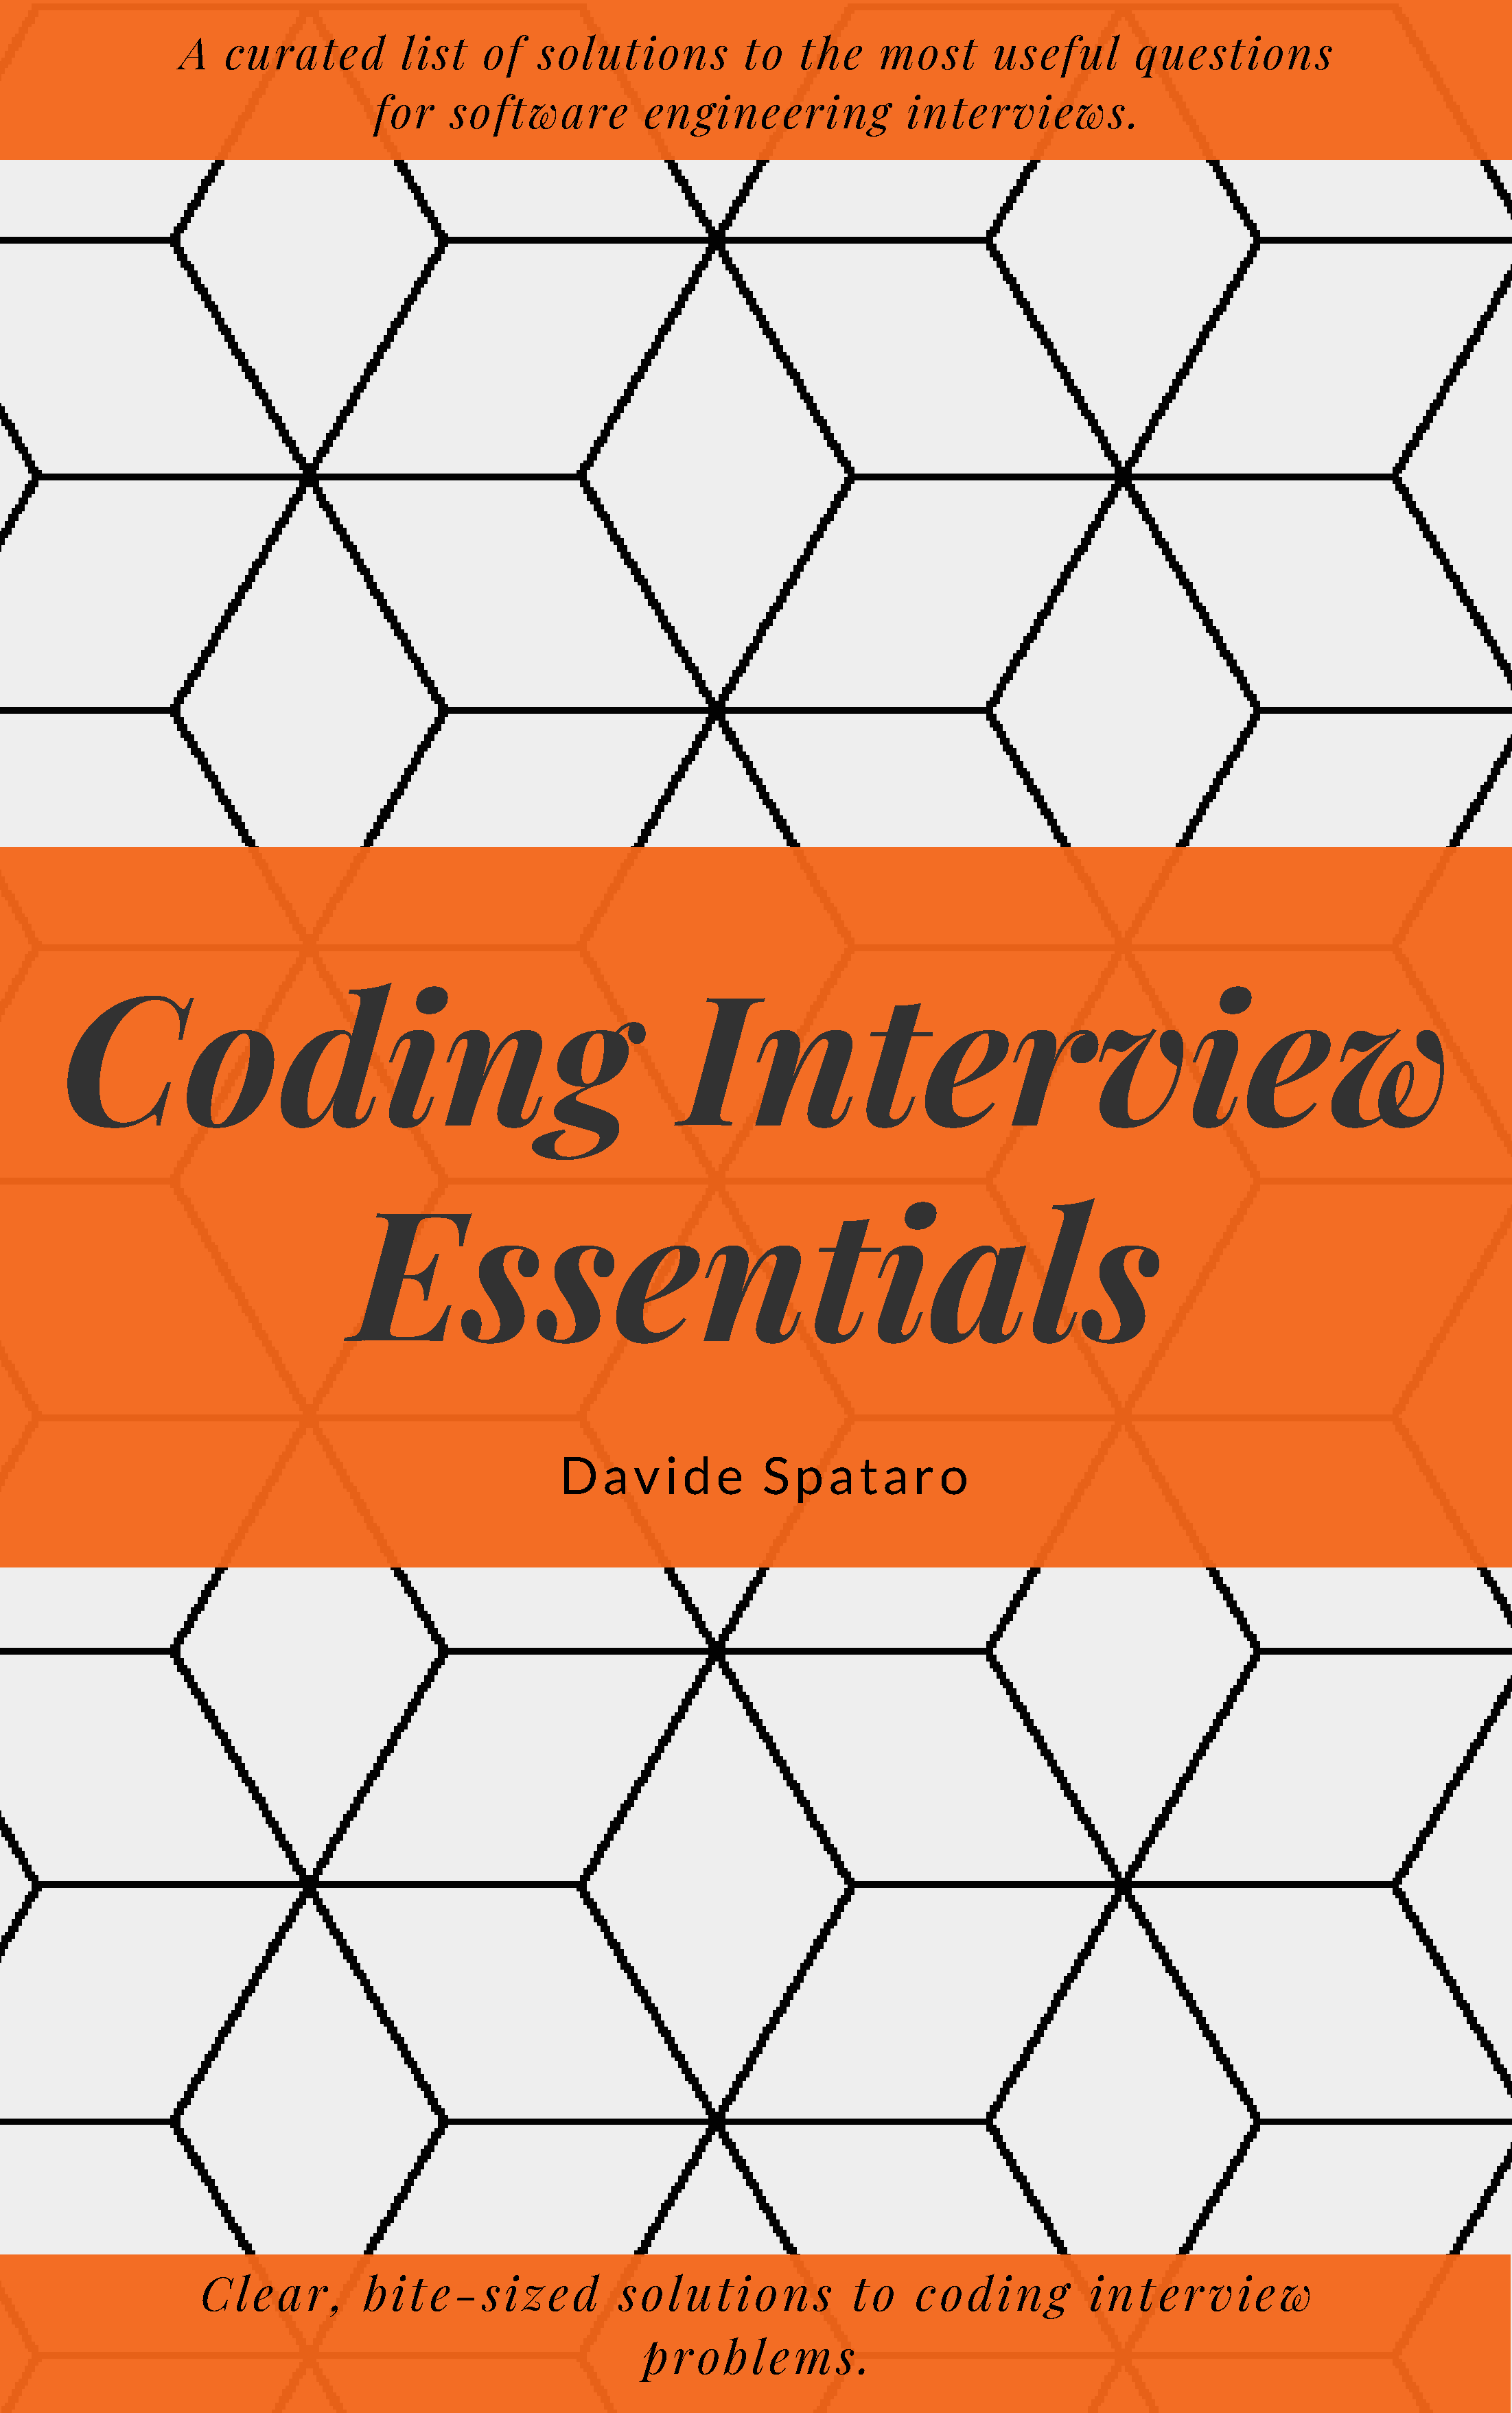
\includepdf[pages=1, fitpaper]{sources/front_cover_image.pdf}
%%\begingroup
%\thispagestyle{empty}
%\begin{tikzpicture}[remember picture,overlay]
%  \coordinate [below=12cm] (midpoint) at (current page.north);
%  \node at (current page.north west)
%  {\begin{tikzpicture}[remember picture,overlay]
%      \node[anchor=north west,inner sep=0pt] at (0,0) {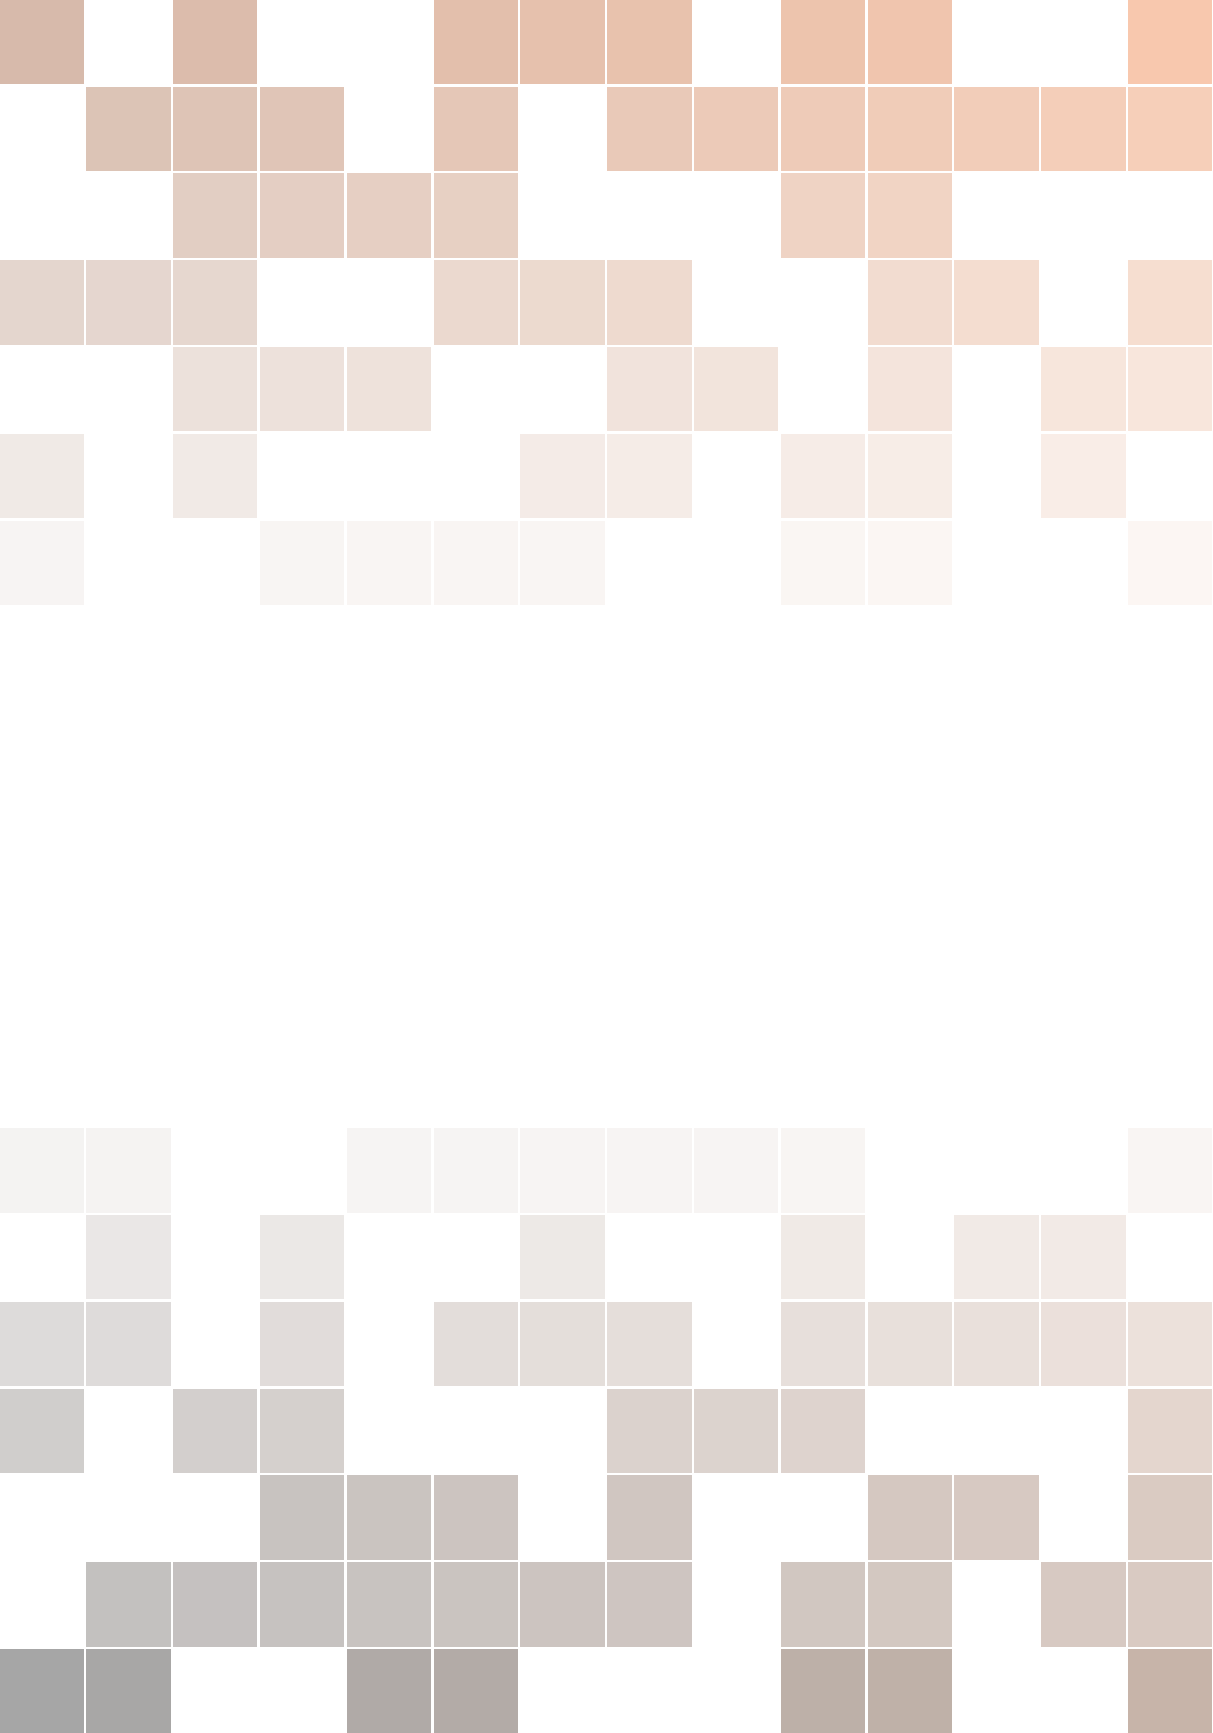
\includegraphics[width=\paperwidth]{images/background}}; % Background image
%\textsl{}
%      \draw[anchor=north] (midpoint) node [fill=ocre!30!white,fill opacity=0.6,text opacity=1,inner sep=1cm]{\Huge\centering\bfseries\sffamily\parbox[c][][t]{\paperwidth}{\centering Coding Interview Essentials\\[15pt] % Book title
%      {\Large - }\\[20pt] % Subtitle
%      {\huge Davide Spataro}}}; % Author name
%    \end{tikzpicture}};
%\end{tikzpicture}
%\vfill
%\endgroup


\includepdf[pages={2},fitpaper=true]{images/book_covers1.pdf}


\usechapterimagefalse % If you don't want to include a chapter image, use this to toggle images off - it can be enabled later with \usechapterimagetrue

%\chapterimage{images/header} % Table of contents heading image

\pagestyle{empty} % No headers

\tableofcontents % Print the table of contents itself

%\lstlistoflistings
%\listoffigures
%\listoftables

\cleardoublepage % Forces the first chapter to start on an odd page so it's on the right

%pagestyle{fancy} % Print headers again
%!TEX root = ../main.tex
%%%%%%%%%%%%%%%%%%%%%%%%%%%%%%%%%%
% Links:
%
% Difficulty:
% Companies: 
%%%%%%%%%%%%%%%%%%%%%%%%%%%%%%%%%%


%\begin{figure}
%   \centering
%   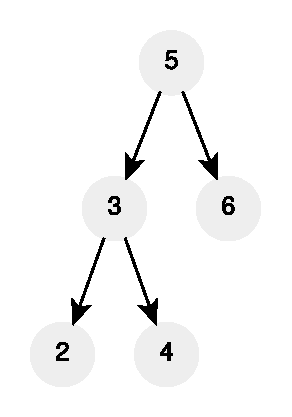
\includegraphics[width=\textwidth]{sources/kth_smallest_in_sorted_matrix/images/example1}
%   \caption[Sample short cpation]{Sample Caption}.
%   \label{fig:kth_smallest_in_sorted_matrix:example1}
%\end{figure}

\chapter{$k^{th}$ smallest element in a sorted matrix}
\label{ch:kth_smallest_in_sorted_matrix}
\section*{Introduction}
\begin{wraptable}{r}{4.5cm}
    \centering
    \begin{framed}  
    \begin{tabular}{|c|c|c|}
    \hline
    1  & 5  & 9  \\ \hline
    10 & 12 & 13 \\ \hline
    12 & 13 & 15 \\ \hline
\end{tabular}%
\caption{Tabular representation of Example \ref{example:kth_smallest_in_sorted_matrix:example1}}
\label{tab:kth_smallest_in_sorted_matrix:example1}
\end{framed}
\end{wraptable} 

One of the most common tool in computer science and engineering in general are rectangular grids of number also known as matrices\footnote{Matrices however are not stored in memory as grids. Computer memory is linear (think of it as an array) and therefore matrices must be mapped into it in some way. Turns out there is not only a single way of performing such a mapping, with the most common ones being \textit{row-major} and \textit{column-major}. The row-major stores each rows one after the other contiguously in memory  while column-major does the same but with columns. The matrix in Example \ref{example:kth_smallest_in_sorted_matrix:exercice1} would be stored as $\{\underbrace{1,5,9}_{\text{row 0}},\underbrace{10,12,13}_{\text{row 1}},\underbrace{12,13,15}_{\text{row 2}}\}$ in a row-major mapping and as $\{\underbrace{1,10,12}_{\text{col 0}},\underbrace{5,12,13}_{\text{col 1}},\underbrace{9,13,15}_{\text{col 2}}\}$as column-major.}. The data they  contain can represent many things, from mathematical set of linear equations to algorithm for compression of images and videos or graphs.

In this chapter, we are not going to worry about all of those fancy applications of matrices, and instead, we will focus on a much simpler problem on a class of matrices of integers with the property of having rows and columns sorted. The task we need to perform on such a matrix is one that is easily explained: we have to find the $k^{th}$ smallest number among \textbf{all} values in the matrix.
This is one such problem for which we will be able to find a working solution straight away, but coming up with a more efficient time and space solution is way more complicated. 
On top of that, the naive solution differs conceptually quite a bit from the faster ones and that further complicates things, especially during an interview. Most of us, once the naive solution is found, are naturally driven towards optimizing it rather than trying to think about a radically different way to approach the problem which, as we will see below, is key to finding solutions with better asymptotic complexity.



\section{Problem statement}
\begin{exercise}
\label{example:kth_smallest_in_sorted_matrix:exercice1}
Write a function that, given an square matrix $M$ of size $n$  where each of individual row and column is sorted in ascending order and an integer $1 \leq k \leq n^2$
returns the $k^{th}$ smallest element in $M$.


You can assume the elements of $M$ to be always in the range $[0,n^2]$.

    %example1
    \begin{example}
        \label{example:kth_smallest_in_sorted_matrix:example1}
        \hfill \\
        Given $M=\{\{1,5,9\},\{10,12,13\},\{12,13,15\}\}$ (as shown in Table \ref{tab:kth_smallest_in_sorted_matrix:example1}) and $k=8$ the function returns $13$.
    \end{example}
\end{exercise}




\section{Clarification Questions}

\begin{QandA}
    \item Can we assume the input to be always valid i.e. having rows and column sorted?
    \begin{answered}
        \textit{Yes, there is no need to perform any input validation whatsoever.}
    \end{answered}
    
    \item Can $M$ contains duplicates?
    \begin{answered}
        \textit{Yes.}
    \end{answered}
    
\end{QandA}

\subsection{Brute-force}
\label{kth_smallest_in_sorted_matrix:sec:bruteforce}
A quick solution to this problem would be to copy into a vector \textbf{all} elements of $M$. If can sort this vector we will have the answer at location  $k-1$. 
This solution, implemented in Listing \ref{list:kth_smallest_in_sorted_matrix:bruteforce}, is simple, easy to explain and implement, and most importantly is correct. 

\lstinputlisting[language=c++, caption={Naive brute-force solution.},label=list:kth_smallest_in_sorted_matrix:bruteforce]{sources/kth_smallest_in_sorted_matrix/kth_smallest_in_sorted_matrix_solution1.cpp}

The code works by copying every single row of $M$ into a temporary array \inline{M_linear} that we then proceed to sort. We can notice how in reality \inline{M_linear} is not really sorted fully, but only partially by using \inline{std::partial_sort}\cite{cit::std::partialsort} (see Section \ref{sec:find_k_closest_in_array:sorting} for another problem where we used this type of sorting) which is called in such a way that the smallest $k$ elements of $M$ are moved to the front of \inline{M_linear} and are properly sorted leaving the rest of \inline{M_linear} unsorted. That is OK because we do not really care about anything but the $k^{th}$ smallest elements.
We use \inline{std::partial_sort} as this way the overall complexity of this approach is dependent on $k$ instead of the total number of elements in $M$. When $k << |M|$ this can result in measurable performance improvements. However, this does not really change the overall time final asymptotical complexity as $K$ can be as big as $|M|$.
The time and space complexities are therefore $O(nm\times log(nm)$) and $O(nm)$, respectively, where $nm$ is the number of elements in $M$.

\subsection{Brute-force improved}
\label{kth_smallest_in_sorted_matrix:sec:bruteforce_constant_space}
In Section \ref{kth_smallest_in_sorted_matrix:sec:bruteforce} we solved the problem by pure brute-force and we did not take advantage of the fact that rows and columns are sorted to begin with. 
A possible way we can use this fact to our advantage is to use two pointers \inline{rightPtr}, and \inline{downPtr} to navigate rows and columns, respectively. \inline{rightPtr} will always move to the right (thus inspecting rows) and \inline{downPtr} will go downwards to take care of columns. 
Our claim is that we can move these two pointers one at a time by advancing the one pointing to the smallest element, and visit $M$ respecting the total order of its elements.

First of all, we should notice that the smallest element will always be at the top-left corner (location $(0,0)$ in $M$).
If we initialize them so that \inline{rightPtr=(0,1)} and \inline{downPtr=(1,0)}, then we know that the \nth{1} smallest element is pointed by \inline{downPtr} and the \nth{2} smallest is the smallest between  \inline{rightPtr} and \inline{downPtr}. Whenever a pointer points to the next smallest element, we move it in its prefeered direction (\inline{rightPtr} to the right and \inline{downPtr} downwards). Of course when a pointer reached the limit of the matrix we make sure to move it either to the next row or column and we make sure to make it start so that we avoid cells that have been already visited. Given \inline{downPtr = (p,q)}, when we need to wrap around \inline{rightPtr = (x,y)} we can move it to \inline{(x+1,q+1)} i.e. to the next row, but avoiding looking at any column that have been already looked by \inline{downPtr}. Similarly, when we need to wrap around \inline{downPtr = (p,q)} we make sure to avoid rows already taken into account by \inline{rightPtr} by setting it to \inline{rightPtr = (x+1,q+1)}. 

If we continue to move these pointers then, after we have moved them $k^{th}$ times we know for sure that one of the two pointers points to the final answer and in particular, the smallest of the two is the value we need.
Figure \ref{fig:kth_smallest_in_sorted_matrix:visitall} shows how this work using the instance in Example \ref{example:kth_smallest_in_sorted_matrix:example1}.

\begin{figure}
    \centering
    \begin{subfigure}[t]{0.32\textwidth}
        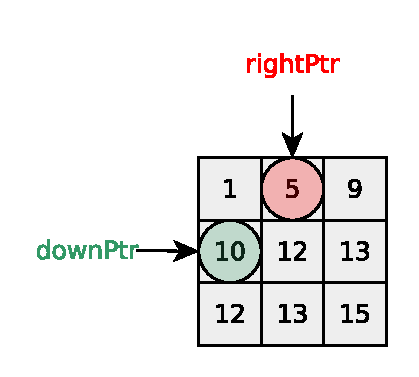
\includegraphics[width=1\linewidth]{sources/kth_smallest_in_sorted_matrix/images/visit1}
        \caption{}
        \label{fig:kth_smallest_in_sorted_matrix:visit1}
     \end{subfigure}
    \hfill
    \begin{subfigure}[t]{0.32\textwidth}
        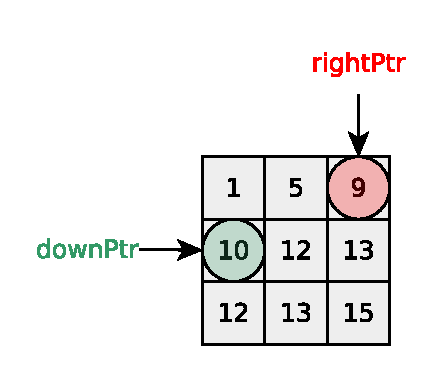
\includegraphics[width=1\linewidth]{sources/kth_smallest_in_sorted_matrix/images/visit2}
        \caption{}
        \label{fig:kth_smallest_in_sorted_matrix:visit2}
     \end{subfigure}
     \hfill
    \begin{subfigure}[t]{0.32\textwidth}
        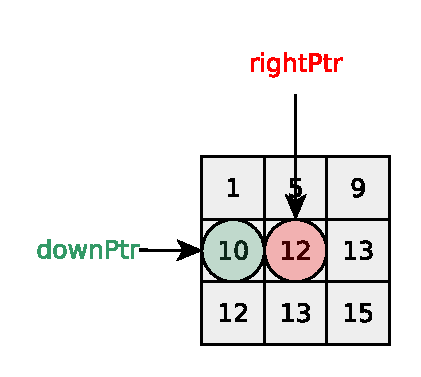
\includegraphics[width=1\linewidth]{sources/kth_smallest_in_sorted_matrix/images/visit3}
        \caption{}
        \label{fig:kth_smallest_in_sorted_matrix:visit3}
     \end{subfigure}
     \hfill
    \begin{subfigure}[t]{0.32\textwidth}
        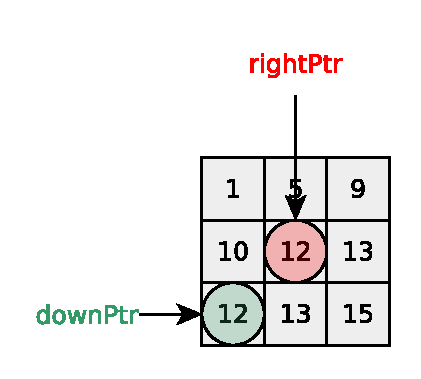
\includegraphics[width=1\linewidth]{sources/kth_smallest_in_sorted_matrix/images/visit4}
        \caption{}
        \label{fig:kth_smallest_in_sorted_matrix:visit4}
    \end{subfigure}
    \hfill
    \begin{subfigure}[t]{0.32\textwidth}
        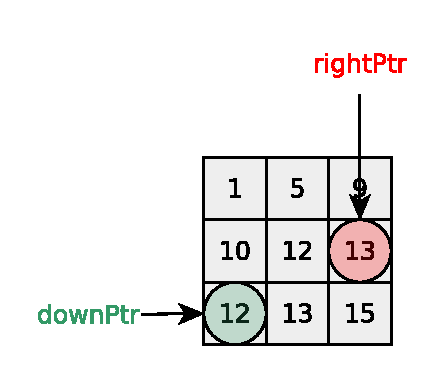
\includegraphics[width=1\linewidth]{sources/kth_smallest_in_sorted_matrix/images/visit5}
        \caption{}
        \label{fig:kth_smallest_in_sorted_matrix:visit5}
    \end{subfigure}
    \hfill
    \begin{subfigure}[t]{0.32\textwidth}
        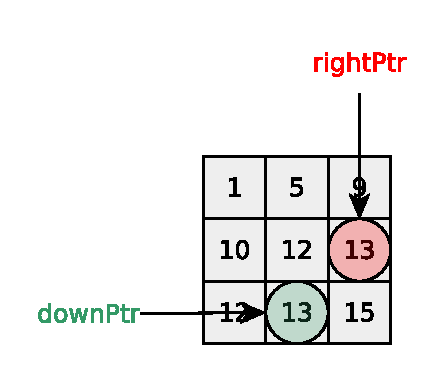
\includegraphics[width=1\linewidth]{sources/kth_smallest_in_sorted_matrix/images/visit6}
        \caption{}
        \label{fig:kth_smallest_in_sorted_matrix:visit6}
    \end{subfigure}
    \hfill
    \begin{subfigure}[t]{0.32\textwidth}
        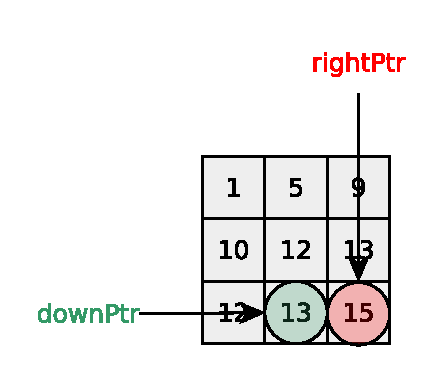
\includegraphics[width=1\linewidth]{sources/kth_smallest_in_sorted_matrix/images/visit7}
        \caption{}
        \label{fig:kth_smallest_in_sorted_matrix:visit7}
    \end{subfigure}
    
    

     \caption[Execution Listing \ref{list:kth_smallest_in_sorted_matrix:bruteforce_improved} on Example \ref{example:kth_smallest_in_sorted_matrix:example1}]{Execution Listing \ref{list:kth_smallest_in_sorted_matrix:bruteforce_improved} on Example \ref{example:kth_smallest_in_sorted_matrix:example1}. The pointers are initialized as shown in Figure \ref{fig:kth_smallest_in_sorted_matrix:visit1}. We then compare them and move \inline{rightPtr} to the right because it is the smallest among the two of them. Next we move it again as shown in Figure \ref{fig:kth_smallest_in_sorted_matrix:visit2} because the value it points to (i.e. $9$) is still smaller than the value pointed by \inline{downPtr}. We cannot move \inline{rightPtr} to the right as it would break the boundaries of the matrix and we therefore move it one row down but we carefully place it a column to the right of the column \inline{downPtr} is at (because \inline{downPtr} is taking care of that column). After that, in Figure \ref{fig:kth_smallest_in_sorted_matrix:visit4} we can see that  \inline{downPtr} is moved. At this point both pointers point to cells containing the same value. When a case like this happens we always choose to move \inline{rightPtr}. In Figure \ref{fig:kth_smallest_in_sorted_matrix:visit5} we see that \inline{downPtr} is moved again. Notice that, because we could not move it downwards, we moved it one column to the right and to a row below \inline{rightPtr}'s row. Up at this point we moved pointers $7$ times if we also consider cell $(0,0)$ that we skipped entirely. We only need to move it once more to be able to find the \nth{8} smallest. This last step is shown in Figure \ref{fig:kth_smallest_in_sorted_matrix:visit7} where \inline{rightPtr} is moved one row below and one column to the right of \inline{downPtr} column coordinate, finally landing in the last cell.}
      \label{fig:kth_smallest_in_sorted_matrix:visitall}
\end{figure}

Notice that there could be a case where it is impossible to move a pointer any further as it would go completely outside the boundaries of the matrix in both directions. When this happens, we should simply continue moving the other pointer and keep counting\footnote{We can think of this case as if the exhausted pointer would be always pointing to imaginary cells of infinite value.}.

An implementation of this idea is shown in Listing \ref{list:kth_smallest_in_sorted_matrix:bruteforce_improved}.

\lstinputlisting[language=c++, caption={Brute-force solution using constnat space.},label=list:kth_smallest_in_sorted_matrix:bruteforce_improved]{sources/kth_smallest_in_sorted_matrix/kth_smallest_in_sorted_matrix_solution2.cpp}

The main driver function, \inline{kth_smallest_in_sorted_matrix_brute_force_constant_space}, contains a bunch of loos with the first, being the main one. We can see there how \inline{downPtr} and \inline{rightPtr} are compared first and the smallest of the two is moved. In order to move them, two auxiliary functions are used: \inline{advanceDown} and \inline{advanceRight}. These functions make sure the pointers are moved properly so that if necessary the wrapping around described above is enforced. We can also notice that they return a boolean value which indicates whether the movement resulted in the pointer going outside the boundary of the matrix.
This boolean value is used to break out of the main loop in \inline{kth_smallest_in_sorted_matrix_brute_force_constant_space} and when this happens to decide which pointer needs to be moved further. If \inline{downPtr} went overboard the matrix then we continue moving \inline{rightPtr} and the other way round if \inline{rightPtr} went overboard. If we reach the end of the first main, then only the body of one of the two subsequent \inline{while} can be executed.

The time and space complexities of this approach are $O(nm)$ and $O(1)$, respectively, with $nm$ being the total number of cells in $M$.

\subsection{Binary Search}
\label{kth_smallest_in_sorted_matrix:sec:binarysearch}
So far, all the solutions we described are based on explicitly sorting the values of $M$. The first by literally sorting them and the second by performing a \quotes{in-order} visit (borrowing the terminology from binary search trees) of $M$. The issue with this approach is that we cannot get away with the fact we might need to end up visiting the entire matrix. We have a lower bound on the time complexity we can reach with any solution based on spelling out the values of $M$ in an ordered fashion: $O(nm)$.

But what if we try to guess what the value of the $k^{th}$ smallest could be and then check if that is indeed the right answer? The guessing part can be carried out using binary search and we know that we will not need more than $O(log(U))$ where $U$ is the difference between the smallest and largest element of $M$ (which are for sure places at cells $(0,0)$ and $(n-1.m-1)$).
However, guessing the number is only part of the story. Once we have a number, we must check that whether it can indeed be the answer or for sure it is not. 
We know that the $k^{th}$ element of $M$ is a value for which there are $k-1$ smaller or equal elements in $M$. We can use this definition to validate our guess. All we have to do is to visit $M$ and count the number that is lower or equal to our guess. However, doing it naively will actually cost us $O(nm)$ as we must look at every cell of $M$! This would result in a worse overall time complexity than the brute-force solution discusses above as we would perform $O(log(U))$ steps each costing $O(nm)$.

However, we can use the fact that rows and columns are sorted in order to speed up this coutning step.
The idea is that, if we want to count how many elements in $M$ are smaller than a given value $x$, we can start from row $0$ and column $m-1$ (the rightmost column). We can check each cell of this row $(0,m-1),(0,m-2),\ldots,(0,p_0 \leq m-1)$ , up until we found an element that is lower or equal than $x$ i.e. $M[0][p_0] \leq x$. At this point, we know for sure that all $p_0$ elements on row $0$ before and including the one at column $p_0$  are smaller than $x$ because we rely on the rows being sorted!

We can now move onto the row $1$ but this time we are not going to start again from the column $m-1$ but, instead, we start our search from column $p_0$.
 The reason is that also columns are sorted and, if a cell at row $0$ in a column to the right of $p_0$ is greater than $x$, so is a cell in any column greater than $p_0$ in \textbf{all} rows below $0$.
We continue processing row $1$ until we find (again) an element that is smaller or equal to $x$. Say we found one at index $p_1 < p_0$. Similarly, with what happened for row $0$ also in this case we can conclude that we have found $p_1$ more elements smaller than $x$ and move on to the next row. 
For the row $2$ we will start our search from column $p_1 \leq p_0$. 

These steps can continue up until either we found a row $i$ for which there are no elements smaller than $x$ i.e. $p_i < 0$ or we have inspected every row of $M$.
Eventually, we will know exactly how many elements are smaller than $x$ in $M$ and we can use this information to adjust our binary search-driven guess of $x$.
In particular, we must make sure our next guess is higher or lower than $x$ depending on whether the number of elements in $M$ smaller than $x$ is smaller or higher (or equal) than $k$, respectively.

Notice that if we find that the number of elements smaller than $M$ is exactly equal to $k$ we cannot immediately conclude $x$ is our answer as $x$ could not even be an element of $M$! However eventually, the binary-search range will be narrowed down to only one value, and at that point, we will be assured that such value is indeed a value in $M$.

Listing \ref{list:kth_smallest_in_sorted_matrix:bs} shows an implementation of this idea.

\lstinputlisting[language=c++, caption={Solution using binary search.},label=list:kth_smallest_in_sorted_matrix:bs]{sources/kth_smallest_in_sorted_matrix/kth_smallest_in_sorted_matrix_solution3.cpp}

The code has a classical binary-search structure with the variables \inline{l} and \inline{r} containing the lower and upper bound of the search space, respectively. At each iteration, we take a guess at the middle of this range (variable \inline{mid}) and we then simply call the function \inline{count_less_or_equal} that, as the name suggests counts the number of values lower or equal than \inline{mid} in $M$ by using the approach described above.
We use the retured value of this function to shrink the search space either to the left (by setting \inline{l=mid}) or to the right (\inline{r=mid+1}). Notice that, when \inline{count_less_mid} is higher or equal than $k$ we do not exclude \inline{mid} from the search space as it might very well be that \inline{mid} is our answer after-all (if \inline{count_less_mid==k} and \inline{mid} is in $M$).

Eventually \inline{l==r} and we can rest assured that \inline{l} contains the value of an actual element of $M$. 
Imagine we are in a situation where every element in $[l,r]$ yields a \inline{count_less_mid} of exactly $k$. When this happens we know for sure that only $l$ is an actual value contained in $M$ as if this was not the case then it would be impossible for another element $g$ in the range $[l,r]$ to still have $k$ elements smaller than $g$ itself as $l$ is smaller than $g$ and therefore the total count for $g$ would be $k+1$.

The complexity of this approach is $O((n+m)log(U))$ as the function \inline{count_less_or_equal} runs in $O(n+m)$ steps. The space complexity is $O(1)$.


%%%%%%%%%%%%%%%%%%%%%%%%%%%%%%%%%%%%%%%%%%%%
%               Appendices
%%%%%%%%%%%%%%%%%%%%%%%%%%%%%%%%%%%%%%%%%%%%

\chapter{Appendices}
%% @Author: Davide Spataro
% @Date:   2020-10-25 
% @Last Modified by:   Davide Spataro
% https://www.topcoder.com/community/competitive-programming/tutorials/dynamic-programming-from-novice-to-advanced/
% file:///home/knotman/Downloads/DYNAMIC_PROGRAMMING_-_ITS_PRINCIPLES_APPLICATIONS_.pdf
% http://smo.sogang.ac.kr/doc/bellman.pdf 
\section*{Dynamic Programming}
\label{sect:appendix:DP}

Dynamic programming (DP) is a popular technique for solving a certain class of
optimization problems efficiently and is accredited to the American Scientist
Richard Bellman\cite{bellman1954}. He conied the term DP in the context of
solving problems involving a serie of best decision one after the other. 
The word \textit{programming} can be a bit deceiving for
computer scientist of programmers in general but it has really little to do with
computer programming and it is infact intended as a set of rules to 
follow to solve a certain problem and it is refeered specifically to the
solution to find an optimal military schedule for logistics (and has more or
less the same meaning as linear programming or linear optimization).  These rules can of course be coded and
executed by a computer but can be easily followed on paper for instance. 
Dynamic programming is better thought as an optimization approach rather than an
method or framework where a complex optimization problem is transformed into a sequence of
smaller (and simpler) problems. The very essence of DP is its multi-stage
optimization procedure. DP does not provide directly with the
instruction on how to solve a particular problem, but instead provides a general
framework that requires creativity and non trivial effort/insights so that a
problem formulation can be adapted and casted within the DP framework bounds.
This is possibly the reason why DP is considered a rather hard topic and it is
particularly feared during interviews. 

This chapter is not intended to be a full treatement of DP, and we will
introduce and describe it to the level that is necessary to understand and
better tackle DP interview problems. For a more comprenshive material on DP
please refer to \cite{bellman1954, cormen2009}.

The gist of the DP approach is that we aim at breaking down a problem into
simpler sub-problems recursively. If it is possible to do so, then the problem
at hand is said to have the \textbf{optimal substructure} property i.e. it can
be solved by using optimal solution to subproblems. But having the optimal
substructure property alone is not enough to prefer a DP approach to another
when trying to solve the same problem. This is because DP really shines when a
problem also exposes the \textbf{overlapping subproblems} property i.e. when the
subproblems are reused several times. A classic example if the
Fibonacci Sequence. In order to calculate $F(n)$ we need to solve two subproblems:
$F(n-1)$ and $F(n-2)$ and adding them up. But for solving $F(n-1)$ we need to
solve $F(n-2)$ \textbf{again}. The value for the subproblem $F(n-2)$ is thus
reused and this makes the Fibonacci problem exposed the optimal substructure
property. 
Dynamic programming takes care of this fact by making sure of solving each
subproblem only once. Usually this can be achieved into two ways:
\begin{description}
    \item [Top-down] This is usually the easiest of the two, by being a direct
    derivation from the recursive formulation of the problem. If the problem can
    be formulated recursively in terms of solution then solution to subproblems
    can be \textit{memoized}\footnote{From the latin word \textit{memorandum}
    which means to be remembered. It is basically a way of remembering the
    result of a function for a certain set of inputs call by storing it in a
    cache.} in a cache. 
    When a subproblem is reused then the
    (potentially expensive) recursive call is avoided and the cached result is
    returned instead. 
    \item [Bottom-up] We can try to reformulate the problem by twisting and
    massaging  the  recursive formulation so that the subproblems are solved
    first (thus effectively removing the recursion) and build the solution to
    the bigger problem from the bottom. This is usually done by working in a
    sort of tabular form where entries of the table for larger problems are
    filled by using  entries for solution to smaller problems that we have
    already solved. For instance, when solving the problem of finding the
    $10^{th}$ Fibonacci number $F(10)$, we can start from the known values for
    $F(0)$ and $F(1)$ and working our way up to $F(2)$  by using $F(1)$ and
    $F(2)$. Once F(2) is ready we can move up to F(3), and so on when we have
    the values for $F(8)$ and $F(9)$ we proceed with calculating $F(10)$.
\end{description}

DP has found application in many field of science such as Control theory,
Bioinformatics AI and operations research. There are a number of problems in
computer science that can be solved by using DP such as the 
\begin{itemize}
    \item Longest Common (or increasing) Subsequence
    \item Weighted Interval Scheduling
    \item Chain Matrix Multiplication
    \item Subset sub
    \item String edit distance
    \item Coin change
    \item 0/1 knapsack problem
    \item Graph shortest path
\end{itemize}

In the next section we will shortly review a number of DP problem focusing on
the key ideas that allow a problem to be approached and solved  using DP.

\subsection*{Fibonacci Sequence}
Computing the $n^{th}$ number of the Fibonacci sequence is probably one of the
most common introductionary example of DP. The Fibonacci sequence recursive
formulation is ready to be solved using a top-down DP approach. Listing
\ref{list:app:dp:canonical} shows a C++ function that calculated the $n^{th}$ Fibonacci
number.
\lstinputlisting[language=c++, caption={Canonical recursive C++ implementation of a function returning the $n^{th}$ Fibonacci number.},label=list:app:dp:canonical]{/home/dspataro/git/algorithm_articles/sources/appendices/fibonacci_canonical.cpp}
Notice that for instance when $F(6)$ a call tree is produced where the same call
is repeated more than once as shown in the list below. $F(2)$ has been
calculated $5$ times!
\begin{itemize}
    \item $F(6) = F(5)+F(4)$
    \item $F(6) = (F(4)+F(3)) + (F(3)+F(2))$
    \item $F(6) = ((F(3)+F(2))+(F(2)+F(1))) + ((F(2)+F(1))+(F(1)+F(0)))$
    \item $F(6) = (((F(2)+F(1))+(F(1)+F(0)))+((F(1)+F(0))+F(1))) + (((F(1)+F(0))+F(1))+(F(1)+F(0)))$
    \item $F(6) = ((((F(1)+F(0))+F(1))+(F(1)+F(0)))+((F(1)+F(0))+F(1))) + (((F(1)+F(0))+F(1))+(F(1)+F(0)))$
\end{itemize}

Listing \ref{list:app:dp:fib} can be improved dramatically if we memoize the function calls
that have been already calculated. This way no duplicate work is done. W.r.t the
previous example, from the second time the value of $F(2)$ is needed, no
additional work is done, as the value in the cache is returned.
\lstinputlisting[language=c++, caption={Canonical recursive top-down Dynamic Programming C++ implementation of a function returning the $n^{th}$ Fibonacci number.},label=list:app:dp:fib]{/home/dspataro/git/algorithm_articles/sources/appendices/fibonacci_dp_top_down.cpp}

%\section{Prefix sum}
\label{sect:appendix:prefix_sum}
In computer science, the prefix sum, cumulative sum, inclusive scan, or simply scan of a sequence of numbers x0, x1, x2, ... is a second sequence of numbers y0, y1, y2, ..., the sums of prefixes (running totals) of the input sequence:
%% @Author: Davide Spataro
% @Date:   2020-03-30 17:18:14
% @Last Modified by:   Davide Spataro
% @Last Modified time: 2020-03-30 17:28:08
\section{Binary Search}
\label{sect:appendix:binary_search}
\lipsum{1}
\lstinputlisting[language=c++, caption={},label=list:listings:hash_pair]{test/common/hash_pair.h}

\section*{Latencies Reference}
\FloatBarrier
\begin{table}[]
    \centering
    \resizebox{\textwidth}{!}{%
    \begin{tabular}{lllll}
    \hline
    \rowcolor[HTML]{C0C0C0} 
    \multicolumn{1}{c}{\cellcolor[HTML]{C0C0C0}\textbf{Operation}}     & \multicolumn{3}{c}{\cellcolor[HTML]{C0C0C0}\textbf{Latency}}               & \multicolumn{1}{c}{\cellcolor[HTML]{C0C0C0}\textbf{Notes}} \\ \hline
    \rowcolor[HTML]{C0C0C0} 
                                                                       & \textit{\textbf{nano}} & \textit{\textbf{micro}} & \textit{\textbf{milli}} &                                                            \\
    \textit{L1 cache reference}                                        & 0.5                    & 0.000500000             & 0.000000500             & 14 \textbackslash{}times L1 cache                          \\
    \textit{Branch mispredict}                                         & 5                      & 0.005000000             & 0.000005000             &                                                            \\
    \textit{L2 cache reference}                                        & 7                      & 0.007000000             & 0.000007000             &                                                            \\
    \textit{Mutex lock/unlock}                                         & 25                     & 0.025000000             & 0.000025000             &                                                            \\
    \textit{Main Memory Reference}                                     & 100                    & 0.100000000             & 0.000100000             & 20 times L2 cache. 200x L1                                 \\
    \textit{Compress 1K bytes with Zippy}                              & 3000                   & 3.000000000             & 0.003000000             &                                                            \\
    \textit{Send 1K bytes over 1 Gbps network}                         & 10000                  & 10.000000000            & 0.010000000             &                                                            \\
    \textit{Read 4K randomly from SSD*}                                & 150000                 & 150.000000000           & 0.150000000             & $\sim$1GB/sec SSD                                          \\
    \textit{Round trip within same datacenter}                         & 500000                 & 500.000000000           & 0.500000000             &                                                            \\
    \textit{Read 1 MB sequentially from SSD*}                          & 1000000                & 1000.000000000          & 1.000000000             & $\sim$1GB/sec SSD, 4X memory                               \\
    \textit{Disk seek}                                                 & 10000000               & 10000.000000000         & 10.000000000            & 20x datacenter roundtrip                                   \\
    \textit{Read 1 MB sequentially from disk}                          & 20000000               & 20000.000000000         & 20.000000000            & 80x memory, 20X SSD                                        \\
    \textit{Send packet CA-\textgreater{}Netherlands-\textgreater{}CA} & 150000000              & 150000.000000000        & 150.000000000           &                                                           
    \end{tabular}%
    }
    \caption{Latency Comparison Numbers ($\sim$2012). Credit to \url{https://gist.github.com/jboner/2841832}}
    \label{tab:refernce_latencies}
\end{table}
\FloatBarrier


\begin{figure}
	\centering
	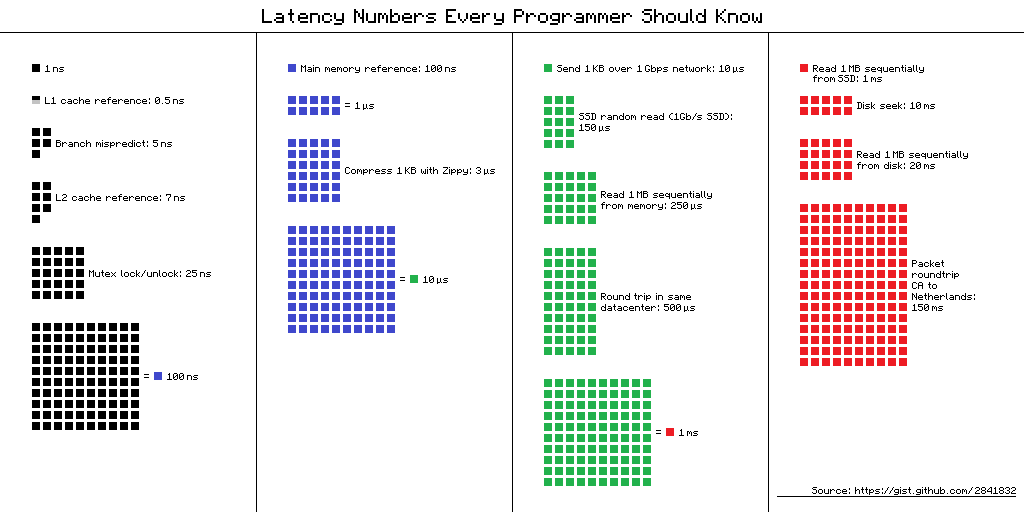
\includegraphics[width=\textwidth]{sources/appendices/images/latencies-refernece.png}
	\caption[]{Humanized visualization of the data in Table 
    \ref{tab:refernce_latencies}}.
	\label{fig:refernce_latencies}
\end{figure}

\FloatBarrier

\vspace{-2cm}
\section*{Data structures Asymptotic complexity cheatsheet}
% Please add the following required packages to your document preamble:
% \usepackage{booktabs}
% \usepackage{multirow}
% \usepackage{graphicx}
% \usepackage[table,xcdraw]{xcolor}
% If you use beamer only pass "xcolor=table" option, i.e. \documentclass[xcolor=table]{beamer}
\begin{table}[!htbp]
    \centering
    \resizebox{\textwidth}{!}{%
    \begin{tabular}{@{}lccccccccc@{}}
    \toprule
                                              & \multicolumn{8}{l}{\textbf{Time Complexities}}                                                                                                                                                                                                                                                                                                                                                  & \multicolumn{1}{l}{\textbf{Space Complexity}}             \\ \cmidrule(l){2-10} 
                                              & \multicolumn{1}{l}{\textbf{Average case}}    & \multicolumn{7}{l}{\textbf{Worst case}}                                                                                                                                                                                                                                                                                                          & \multicolumn{1}{l}{}                                      \\
    \multirow{-3}{*}{\textbf{Data Structure}} & \multicolumn{1}{l}{\textit{\textbf{Access}}} & \multicolumn{1}{l}{\textit{\textbf{Search}}} & \multicolumn{1}{l}{\textit{\textbf{Insertion}}} & \multicolumn{1}{l}{\textit{\textbf{Deletion}}} & \multicolumn{1}{l}{\textit{\textbf{Access}}} & \multicolumn{1}{l}{\textit{\textbf{Search}}} & \multicolumn{1}{l}{\textit{\textbf{Insertion}}} & \multicolumn{1}{l}{\textit{\textbf{Deletion}}} & \multicolumn{1}{l}{\multirow{-2}{*}{\textbf{Worst case}}} \\ \cmidrule(r){1-1}
    Array                                     & \cellcolor[HTML]{009901}$O(1)$               & \cellcolor[HTML]{FFC702}$O(n)$               & \cellcolor[HTML]{FFC702}$O(n)$                  & \cellcolor[HTML]{FFC702}$O(n)$                 & \cellcolor[HTML]{009901}$O(1)$               & \cellcolor[HTML]{FFC702}$O(n)$               & \cellcolor[HTML]{FFC702}$O(n)$                  & \cellcolor[HTML]{FFC702}$O(n)$                 & \cellcolor[HTML]{FFC702}$O(n)$                            \\
    Stack                                     & \cellcolor[HTML]{009901}$O(1)$               & \cellcolor[HTML]{656565}N.A.                 & \cellcolor[HTML]{009901}$O(1)$                  & \cellcolor[HTML]{009901}$O(1)$                 & \cellcolor[HTML]{009901}$O(1)$               & \cellcolor[HTML]{656565}N.A.                 & \cellcolor[HTML]{009901}$O(1)$                  & \cellcolor[HTML]{009901}$O(1)$                 & \cellcolor[HTML]{FFC702}$O(n)$                            \\
    Queue                                     & \cellcolor[HTML]{009901}$O(1)$               & \cellcolor[HTML]{656565}N.A.                 & \cellcolor[HTML]{009901}$O(1)$                  & \cellcolor[HTML]{009901}$O(1)$                 & \cellcolor[HTML]{009901}$O(1)$               & \cellcolor[HTML]{656565}N.A.                 & \cellcolor[HTML]{009901}$O(1)$                  & \cellcolor[HTML]{009901}$O(1)$                 & \cellcolor[HTML]{FFC702}$O(n)$                            \\
    Singly Linked List                        & \cellcolor[HTML]{FFC702}$O(n)$               & \cellcolor[HTML]{FFC702}$O(n)$               & \cellcolor[HTML]{009901}$O(1)$                  & \cellcolor[HTML]{FFC702}$O(n)$                 & \cellcolor[HTML]{FFC702}$O(n)$               & \cellcolor[HTML]{FFC702}$O(n)$               & \cellcolor[HTML]{009901}$O(1)$                  & \cellcolor[HTML]{FFC702}$O(n)$                 & \cellcolor[HTML]{FFC702}$O(n)$                            \\
    Doubly Linked List                        & \cellcolor[HTML]{FFC702}$O(n)$               & \cellcolor[HTML]{FFC702}$O(n)$               & \cellcolor[HTML]{009901}$O(1)$                  & \cellcolor[HTML]{009901}$O(1)$                 & \cellcolor[HTML]{FFC702}$O(n)$               & \cellcolor[HTML]{FFC702}$O(n)$               & \cellcolor[HTML]{009901}$O(1)$                  & \cellcolor[HTML]{009901}$O(1)$                 & \cellcolor[HTML]{FFC702}$O(n)$                            \\
    Hash Table                                & \cellcolor[HTML]{009901}$O(1)$               & \cellcolor[HTML]{009901}$O(1)$               & \cellcolor[HTML]{009901}$O(1)$                  & \cellcolor[HTML]{009901}$O(1)$                 & \cellcolor[HTML]{FFC702}$O(n)$               & \cellcolor[HTML]{FFC702}$O(n)$               & \cellcolor[HTML]{FFC702}$O(n)$                  & \cellcolor[HTML]{FFC702}$O(n)$                 & \cellcolor[HTML]{FFC702}$O(n)$                            \\
    Binary Search Tree                        & \cellcolor[HTML]{32CB00}$O(log_2(n))$        & \cellcolor[HTML]{32CB00}$O(log_2(n))$        & \cellcolor[HTML]{32CB00}$O(log_2(n))$           & \cellcolor[HTML]{32CB00}$O(log_2(n))$          & \cellcolor[HTML]{FFC702}$O(n)$               & \cellcolor[HTML]{FFC702}$O(n)$               & \cellcolor[HTML]{FFC702}$O(n)$                  & \cellcolor[HTML]{FFC702}$O(n)$                 & \cellcolor[HTML]{FFC702}$O(n)$                            \\
    Red-Black Tree                            & \cellcolor[HTML]{32CB00}$O(log_2(n))$        & \cellcolor[HTML]{32CB00}$O(log_2(n))$        & \cellcolor[HTML]{32CB00}$O(log_2(n))$           & \cellcolor[HTML]{32CB00}$O(log_2(n))$          & \cellcolor[HTML]{32CB00}$O(log_2(n))$        & \cellcolor[HTML]{32CB00}$O(log_2(n))$        & \cellcolor[HTML]{32CB00}$O(log_2(n))$           & \cellcolor[HTML]{32CB00}$O(log_2(n))$          & \cellcolor[HTML]{FFC702}$O(n)$                            \\
    Heap                                      & \cellcolor[HTML]{009901}$O(1)$               & \cellcolor[HTML]{656565}N.A.                 & \cellcolor[HTML]{32CB00}$O(log_2(n))$           & \cellcolor[HTML]{32CB00}$O(log_2(n))$          & \cellcolor[HTML]{009901}$O(1)$               & \cellcolor[HTML]{656565}N.A.                 & \cellcolor[HTML]{32CB00}$O(log_2(n))$           & \cellcolor[HTML]{32CB00}$O(log_2(n))$          & \cellcolor[HTML]{FFC702}$O(n)$                            \\ \bottomrule
    \end{tabular}%
    }
    \caption{Asymptotic complexities for a number of data strucutes. For time, both the average and case is reported, while for space only the worst. $O(1) < O(log_2(n)) < O(log_2(n)) < O(n) < O(nlog_2(n) < O(n^2) < O(n^3) \ldots < O(2^n) < O(n!) < O(n^n)$  }
    \label{appendix:ds_complexities}
\end{table}


\begin{figure}
    \centering
\begin{tikzpicture}
    \begin{axis}[
      grid = major,
      clip = true,
      ticks = none,
      width=0.9\textwidth,
      height=0.7\textwidth,
      every axis plot/.append style={very thick},
      axis line style = ultra thick,
      clip mode=individual,
      restrict y to domain=0:40,
      restrict x to domain=0:20,
      axis x line = left,
      axis y line = left,
      domain = 0.00:10,
      xmin = 0,
      xmax = 11,
      ymin = 0,
      ymax = 42,
      xlabel = n,
      ylabel = no. of operations,
      xlabel style = {at={(axis description cs:0.5,-0.1)},anchor=south},
      ylabel style = {at={(axis description cs:-0.08,0.5)},anchor=north},
      label style = {font=\LARGE\bf},
    ]
  \addplot [
      samples=100, 
      color=red,
  ]
  {x^2}node[above,pos=1,style={font=\Large}]{$\mathcal{O}(n^2)$};
  \addplot [
      samples=100, 
      color=blue,
  ]
  {x}node[above,pos=1,style={font=\Large}]{$\mathcal{O}(n)$};
  \addplot [
      samples=100, 
      color=orange,
  ]
  {log2 x}node[above,pos=1,style={font=\Large}]{$\mathcal{O}(\log{}n)$};
  \addplot [
      samples=100, 
      color=black,
  ]
  {x*(log2 x)}node[above,pos=1,style={font=\Large}]{$\mathcal{O}(n\log{}n)$};
  \addplot [
      samples=100, 
      color=magenta,
  ]
  {1}node[above,pos=1,style={font=\Large}]{$\mathcal{O}(1)$};
  \addplot [
      samples=100, 
      color=cyan,
  ]
  {x^(2.2)}node[above,pos=1,style={font=\Large}]{$\mathcal{O}(n^3)$};
  

  \addplot [
    samples=100,
    color=green, 
  ] gnuplot{gamma(x+3)} node[above,pos=1,style={font=\Large}]{$\mathcal{O}(n!)$};

  \addplot [
    samples=100, 
    color=yellow,
]
{2.5*2^x}node[above,pos=1,style={font=\Large}]{$\mathcal{O}(2^x)$};
  
  \end{axis}
  \end{tikzpicture}

  \caption[]{Graph showing the relative growth rates of common function used to describe algorithms.}
  \label{fig:ds_complexities:graph}
\end{figure}
%%%%%%%%%%%%%%%%%%%%%%%%%%%%%%%%%%%%%%%%%%%%
%               BIBLIOGRAPHY
%%%%%%%%%%%%%%%%%%%%%%%%%%%%%%%%%%%%%%%%%%%%

%
%from documentation
%\newacronym[⟨key-val list⟩]{⟨label ⟩}{⟨abbrv ⟩}{⟨long⟩}
%above is short version of this
% \newglossaryentry{⟨label ⟩}{type=\acronymtype,
% name={⟨abbrv ⟩},
% description={⟨long⟩},
% text={⟨abbrv ⟩},
% first={⟨long⟩ (⟨abbrv ⟩)},
% plural={⟨abbrv ⟩\glspluralsuffix},
% firstplural={⟨long⟩\glspluralsuffix\space (⟨abbrv ⟩\glspluralsuffix)},
% ⟨key-val list⟩}

\newacronym{cd}{CD}{compact disk}
\newacronym{utc}{UTC}{Coordinated Universal Time}
%\newacronym{adt}{ADT}{Atlantic Daylight Time}
%\newacronym{est}{EST}{Eastern Standard Time}
 
% Use the acronyms
\gls{utc} is 3 hours behind \gls{adt} and 10 hours ahead of \gls{est}.



%\addcontentsline{toc}{chapter}{\textcolor{ocre}{Glossary}}
%\printglossaries


%Print the glossary

\addcontentsline{toc}{chapter}{\textcolor{ocre}{Bibliography}}
%\chapter*{Bibliography}
%Print the glossary
\printbibliography	
	
%%%%%%%%%%%%%%%%%%%%%%%%%%%%%%%%%%%%%%%%%%%%
%               INDEX
%%%%%%%%%%%%%%%%%%%%%%%%%%%%%%%%%%%%%%%%%%%%	
	\cleardoublepage
	\phantomsection
	\setlength{\columnsep}{0.75cm}
	\addcontentsline{toc}{chapter}{\textcolor{ocre}{Index}}
	\printindex


	%\backmatter

\end{document}
